\documentclass[a4paper]{scrartcl}
\usepackage[utf8]{inputenc}
\usepackage[francais]{babel}
\usepackage{amsmath} % math
\usepackage{amssymb} % math
\usepackage{gensymb} % math
\usepackage[T1]{fontenc}
\usepackage{lmodern}
\usepackage{graphicx}
\usepackage{url}
    \urlstyle{sf}
\usepackage[usenames]{color}
\usepackage{array}
%\usepackage{etex} % chimie
%\usepackage{m-pictex} % chimie
%\usepackage{m-ch-en} % chimie
%\usepackage{lipsum}% pour mettre du texte aléatoire via \lipsum
\definecolor{codeBlue}{rgb}{0,0,1}
\definecolor{webred}{rgb}{0.5,0,0}
\definecolor{codeGreen}{rgb}{0,0.5,0}
\definecolor{codeGrey}{rgb}{0.6,0.6,0.6}
\definecolor{webdarkblue}{rgb}{0,0,0.4}
\definecolor{webgreen}{rgb}{0,0.3,0}
\definecolor{webblue}{rgb}{0,0,0.8}
\definecolor{orange}{rgb}{0.7,0.1,0.1}
\usepackage{caption}
\renewcommand{\familydefault}{\sfdefault}
\date{\today} %\today
%\institute{Cairo-Dock}
\usepackage{listings}        % Pour l'insersion de fichiers de codes sources.
\lstset{
      language=C,
      flexiblecolumns=true,
      numbers=left,
      stepnumber=1,
      numberstyle=\ttfamily\tiny,
      keywordstyle=\ttfamily\textcolor{blue},
      stringstyle=\ttfamily\textcolor{red},
      commentstyle=\ttfamily\textcolor{green},
      breaklines=true,
      extendedchars=true,
      basicstyle=\ttfamily\scriptsize,
      showstringspaces=false
    }
\title{\texttt{LING1113}: Projet 1 : Multiplication de matrices creuses}
\author{\textsc{Matthieu Baerts} \& \textsc{Hélène Verhaeghe}\\Groupe 21}
\begin{document}
\maketitle
% \tableofcontents
\section{Performances du programme}
\subsection{Contexte}
Afin de comparer les performances de notre programme avec une implémentation triviale de matrices pleines (avec un tableau à deux dimensions), nous fournissons avec notre code les deux implémentations. La première se trouve dans \texttt{matrix.c} et la deuxième dans \texttt{matrix\_plain.c}. Concernant les exécutables, lors de l'utilisation de la commande \texttt{make}, deux binaires seront produits: \texttt{matrixprod} et \texttt{matrixprod\_plain}.

\subsection{Mesures réalisées}
Dans les tableaux \ref{tab:plein} et suivants se retrouvent différentes mesures réalisées avec plusieurs matrices allant de 90 à 100 éléments par colonnes et lignes. Dans ces tableaux, nous retrouvons à chaque fois, dans la première colonne, le nombre de matrices à multiplier et dans la seconde, le temps mis pour faire l'entièreté des multiplications. Le temps de calculs avec les matrices pleines ne varie pas en fonction de la composition de la matrice.\\

\begin{table}
    \caption{Calculs avec l'implémentation de matrices pleines}
    \label{tab:plein}
    \begin{center}
        \begin{tabular}{c|c}
            Nombre matrices & Temps (s)\\
            \hline
            2 &        0.015 \\
    3 &        0.016 \\
    4 &        0.027 \\
    5 &        0.020 \\
    10 &        0.043\\
    15 &        0.066 \\
    20 &        0.098 \\
        \end{tabular}
    \end{center}
\end{table}
\begin{table}
    \caption{Calculs avec l'implémentation de matrices creuses, pour des matrices creuses à environ 90\%}
    \label{tab:90}
    \begin{center}
        \begin{tabular}{c|c}
            Nombre matrices & Temps (s)\\
            \hline
            2 &        0.012 \\
    3 &        0.030 \\
    4 &        0.031 \\
    5 &        0.049 \\
    10 &        0.103\\
    15 &        0.160 \\
    20 &        0.220 \\
        \end{tabular}
    \end{center}
\end{table}
\begin{table}
    \caption{Calculs avec l'implémentation de matrices creuses, pour des matrices creuses à environ 95\%}
    \label{tab:95}
    \begin{center}
        \begin{tabular}{c|c}
            Nombre matrices & Temps (s)\\
            \hline
            2 &        0.000\\
    3 &        0.012\\
    4 &        0.020\\
    5 &        0.028\\
    10 &        0.092\\
    15 &        0.148\\
    20 &        0.188\\
        \end{tabular}
    \end{center}
\end{table}
\begin{table}
    \caption{Calculs avec l'implémentation de matrices creuses, pour des matrices creuses à environ 99\%}
    \label{tab:99}
    \begin{center}
        \begin{tabular}{c|c}
            Nombre matrices & Temps (s)\\
            \hline
             2 &         0.000\\
    3 &           0.004\\
    4 &        0.004\\
    5 &       0.004\\
    10 &         0.008\\
    15 &         0.008 \\
    20 &         0.016\\
        \end{tabular}
    \end{center}
\end{table}

La représentation graphique se trouve à la figure \ref{fig:time}.\\

Pour des matrices de tailles variant de 3000 à 3500,  l'implémentation en matrice creuse met environ 4 fois moins de temps que l'implémentation en matrice pleine pour la multiplication de deux matrices: 1.324s pour l'implémentation creuse et 4.940s pour l'implémentation pleine.

\newpage
\section{Utilité de l'implémentation de matrices creuses}
\begin{figure}
    \begin{center}
        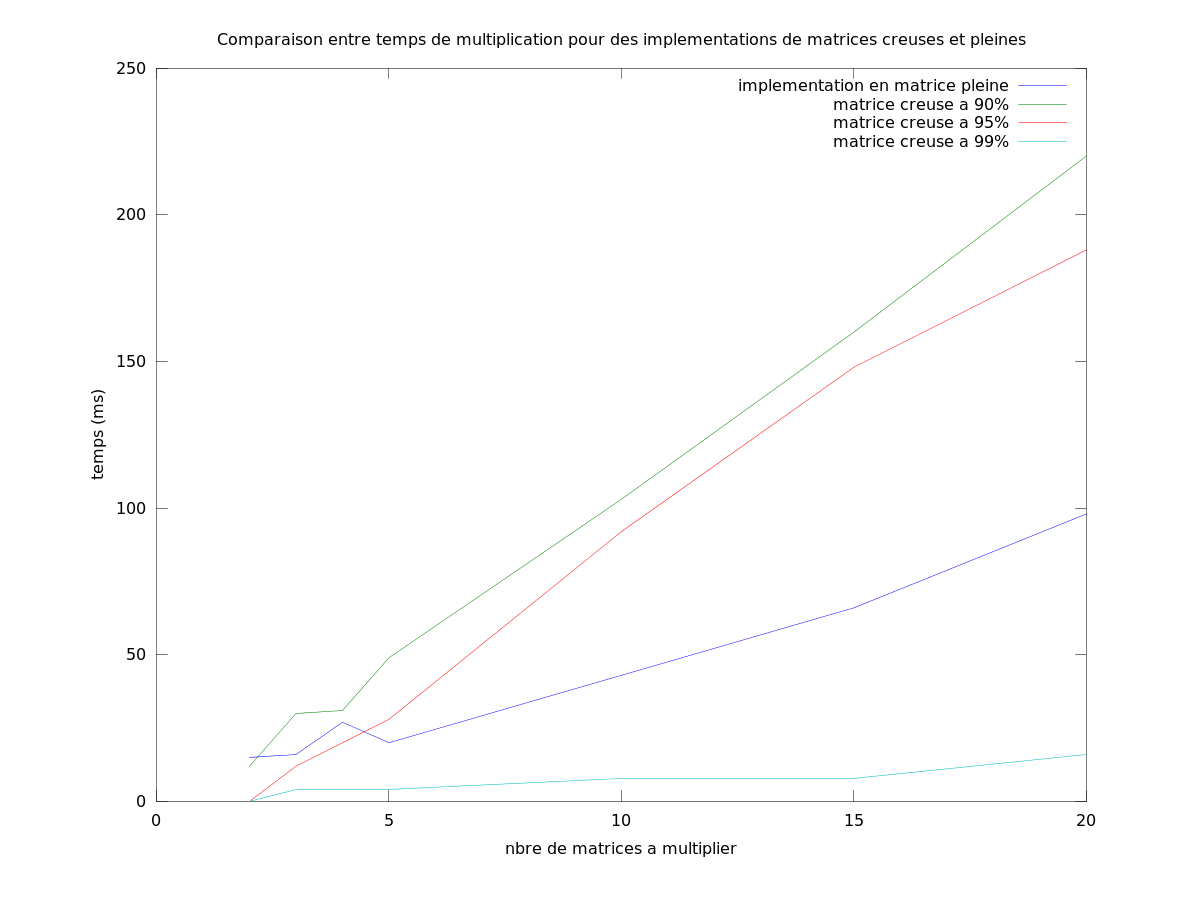
\includegraphics[width=\textwidth]{matrixgraph.png}
        \caption{Représentation graphique des données venant des 3 tableaux précédents}
        \label{fig:time}
    \end{center}
\end{figure}

Comme on peut le voir avec les données des tableaux précédents et surtout du graphe \ref{fig:time} plus les matrices sont creuses, plus notre implémentation devient intéressante. Ceci est tout a fait logique puisque la structure utilisée est beaucoup plus complexe et importante dans notre implémentation comparé à un simple tableau en deux dimensions. Quand il y a peu d'informations dans la matrice (imaginons une matrice diagonale), notre implémentation devient très intéressante car il n'y aura que des calculs avec les éléments existants : si deux matrices de 1000x1000 ne contiennent qu'un seul élément, seuls ces deux éléments seront consultés. La place en mémoire sera également intéressantes dans ce cas de très grandes matrices.
\end{document}
